% -*- root: ../paper.tex -*-

\begin{figure}
\centering
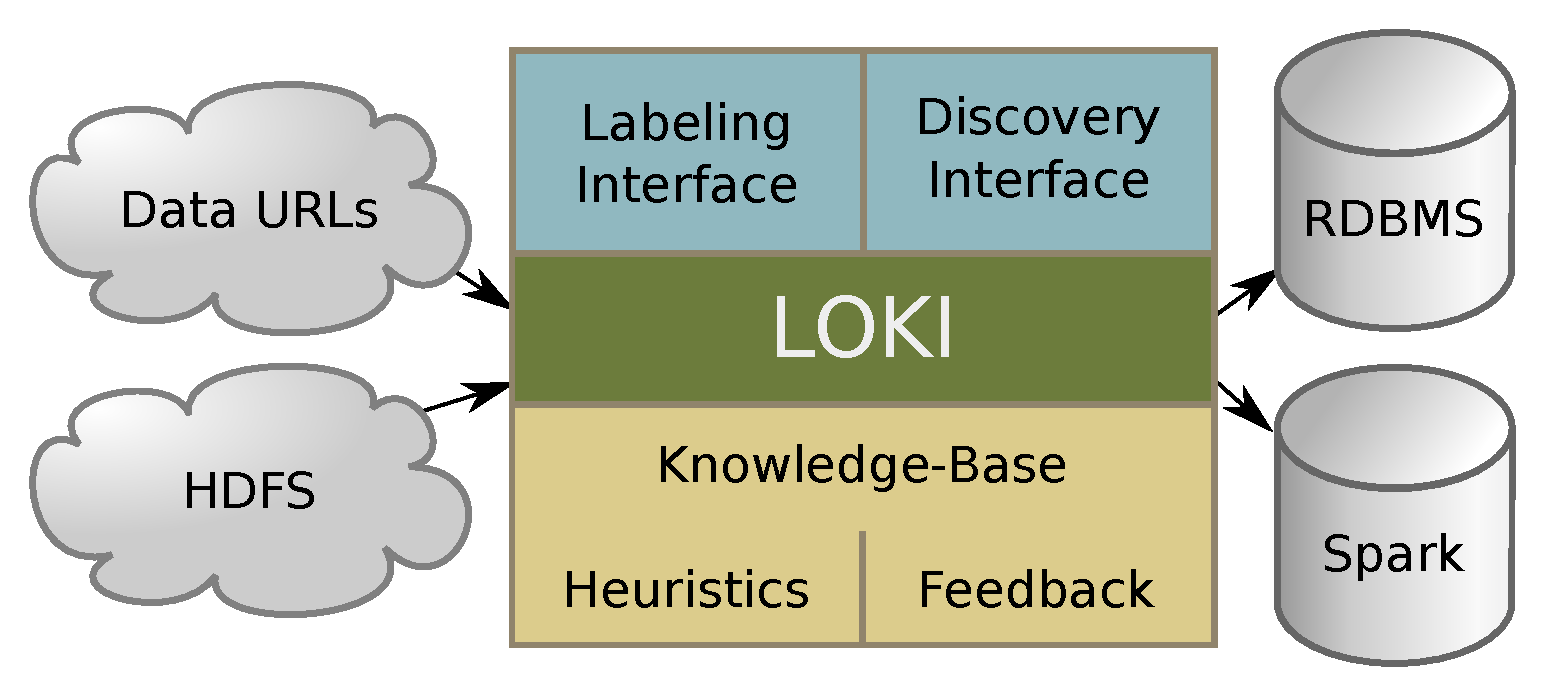
\includegraphics[width=0.8\columnwidth]{graphics/system.pdf}
\caption{System Overview}
\label{fig:overview}
\trimfigurespacing
\vspace*{-1mm}
\end{figure}

The overall goal of \systemname is to streamline the process of developing schemas for existing unlabeled or poorly labeled data sets.  
As illustrated in Figure~\ref{fig:overview}, \systemname lives alongside an existing RDBMS or Spark deployment, and takes as input tabular data in the form of a URL or HDFS file path.
\systemname provides users with two modes of interaction: (1) A \emph{labeling} interface that assists users in assigning names to existing columns of data, and (2) A \emph{discovery} interface that helps users to search for columns representing particular concepts of interest.  
Both interfaces are supported by a knowledge-base that combines expert-provided heuristics, learned characteristics, as well as historical feedback gathered from users about already-loaded datasets.
Once the user has labeled or discovered a sufficient set of columns, \systemname generates appropriate data loading/initialization code (e.g., a \texttt{CREATE TABLE} or Spark DataFrame initializer).  


\subsection{Labeling and Discovery}

We assume that data arrives in unlabeled tabular format.  
An $N$-column input table $T$ consists of a set of rows $t \in T$.
Each row is an indexed list of attribute values $t = \tuple{t[1], \ldots, t[N]}$ with a common schema $sch(T)$.
The columns of $T$, denoted $T_C = \{A_1, \ldots A_N\}$, are the \emph{bag} of values in the projection of the rows of T onto the specified attribute: $A_i \defineeq \bagcomprehension{t[i]}{t \in T}$.
We define the domain of $A$, denoted $dom(A)$ to be the \emph{set} of such values (i.e., $set(T_A)$).  
A \emph{schema} $S$ for $T$ is a list of $N$ \emph{names}, or human interpretable strings $S[1], \ldots, S[N]$ identifying each attribute.
Note that this definition differs slightly from the classical definition of schemas; for us a schema consists only of a name and not the attribute's domain.

\systemname addresses two closely related schema construction problems that we term labeling and discovery queries.
Both types of queries make use of a form of best-fit heuristic matching that we discuss in depth in Section~\ref{sec:knowledgebase}.
Specifically, a \textbf{Labeling} query derives a schema $S$ for a table $T$.
If the user previously provided a names for one of the columns, this name is used in the derived schema.
Otherwise, the best-fit heuristic matching is used.
A \textbf{Discovery} query addresses the dual problem: finding the attribute $A_i$ in a table $T$ most likely to match a given column name.

\subsection{Other Implementation Concerns}
In order to load data into a relational database management system, \systemname needs a way to infer the type (e.g., Numeric, String, or Ordinal) of columns of ingested data.  
For this, we adopt a simple counting-based technique~\cite{yang2015lenses}:
We attempt to parse each value using an array of regular expressions, one for each registered type.
A majority vote of successful parses in a column decides the column's type, with a threshold of 50\% indicating a string column and fewer than 100 distinct values indicating an ordinal.
Admittedly, more advanced techniques that relate columns, for example using functional dependencies, are possible.
However majority vote suffices for most use cases, and as such we leave more interesting type annotation schemes to future work.

Furthermore, \systemname needs to actually load data into the underlying RDBMS.  
We use each platform's native loading scheme: \texttt{DataFrameReader}s on Spark, and native \texttt{LOAD} commands on RDBMSes, with a fall-back to manual \texttt{INSERT} operations if necessary.
As before, more intricate loading options are possible~\cite{DBLP:conf/sigmod/AlagiannisBBIA12,DBLP:conf/cidr/IdreosKM07}, but are beyond the scope of this paper.




